

\chapter{Raspberry PI 3}\label{raspberry-pi-3}

\FILENAME\

\section{Raspbery PI for IOT
(Gregor)}\label{raspbery-pi-for-iot-gregor}

\section{Hardware}\label{hardware}

see hardware page we have

\section{Installation}\label{installation}

\subsection{Erasing the SD Card}\label{erasing-the-sd-card}

Before you can install an OS on your sd card, you must erase it and put
it in the proper format.

\begin{enumerate}
\def\labelenumi{\arabic{enumi}.}

\item
  Insert your sd card into your micro-sd adapter and open Disk Utility
  with a spotlight search.
\item
  In the Disk Utility, right click the name of the sd card and select
  erase.
\item
  Name the sd card and format it as MS-DOS (FAT). Then click erase.

  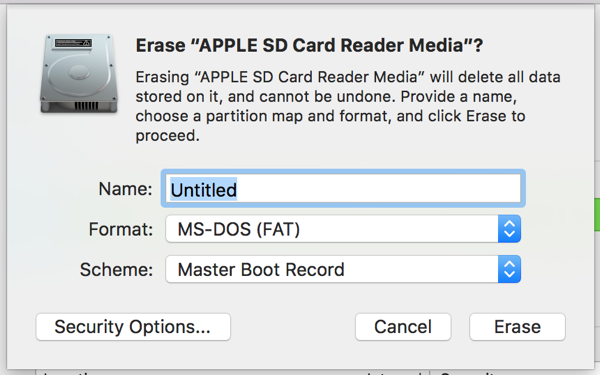
\includegraphics[width=0.5\textwidth]{images/diskutil.png}

\item
  If it does not erase the first time, try again. It sometimes takes
  multiple tries to work.
\end{enumerate}

\subsection{Installation of NOOBS}\label{installation-of-noobs}

NOOBS is an OS that includes Raspian. The official descrition of
Raspbian can be found
\href{https://www.raspberrypi.org/downloads/raspbian/}{here}. It comes
pre-packaged with many useful programming tools, and is easy to use.

\begin{enumerate}
\def\labelenumi{\arabic{enumi}.}

\item
  Download Noobs
  \href{https://www.raspberrypi.org/downloads/noobs/}{here}. This will
  take around 30 minutes.
\item
  Go to your Finder and in Downloads, search for NOOBS.
\item
  Open the NOOBS folder and drag its contents into the sd card in the
  devices section. There should be 20 files and folders in the NOOBS
  folder. The download should take about 3 minutes.
\item
  Once installed, eject the sd card and put it in your raspberry pi.
\item
  Power up your raspberry and you will see a menu like this
\end{enumerate}

\begin{figure}[htb]
\centering
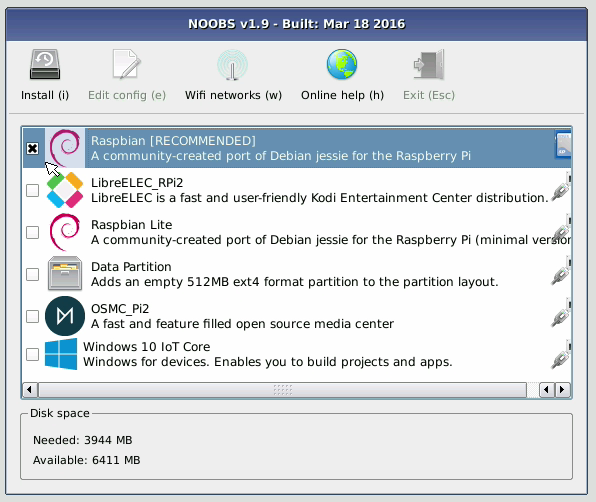
\includegraphics[width=0.5\textwidth]{images/noobs.jpg}
\caption{Noobs}
\end{figure}

\begin{enumerate}
\def\labelenumi{\arabic{enumi}.}
\setcounter{enumi}{5}

\item
  Select Raspbian and click \texttt{Install\ (i)}
\end{enumerate}

\subsection{Installation of Dexter}\label{installation-of-dexter}

The version of Dexter that you want to flash onto your sd card is called
Raspbian for Robots. This is a Raspbian based os that is compatible with
the GrovePi board. It also comes with pre-installed Dexter Industries
software.

\begin{enumerate}
\def\labelenumi{\arabic{enumi}.}

\item
  First, download the most recent Dexter\_Industries\_jessie.zip file
  from
  \href{https://sourceforge.net/projects/dexterindustriesraspbianflavor/}{here}.
\item
  Once the file has downloaded, uncompress it and insert your sd card
  into the micro-sd adapter.
\item
  Open etcher and flash the uncompressed jessie image onto the sd card.
\end{enumerate}

\begin{figure}[htb]
\centering
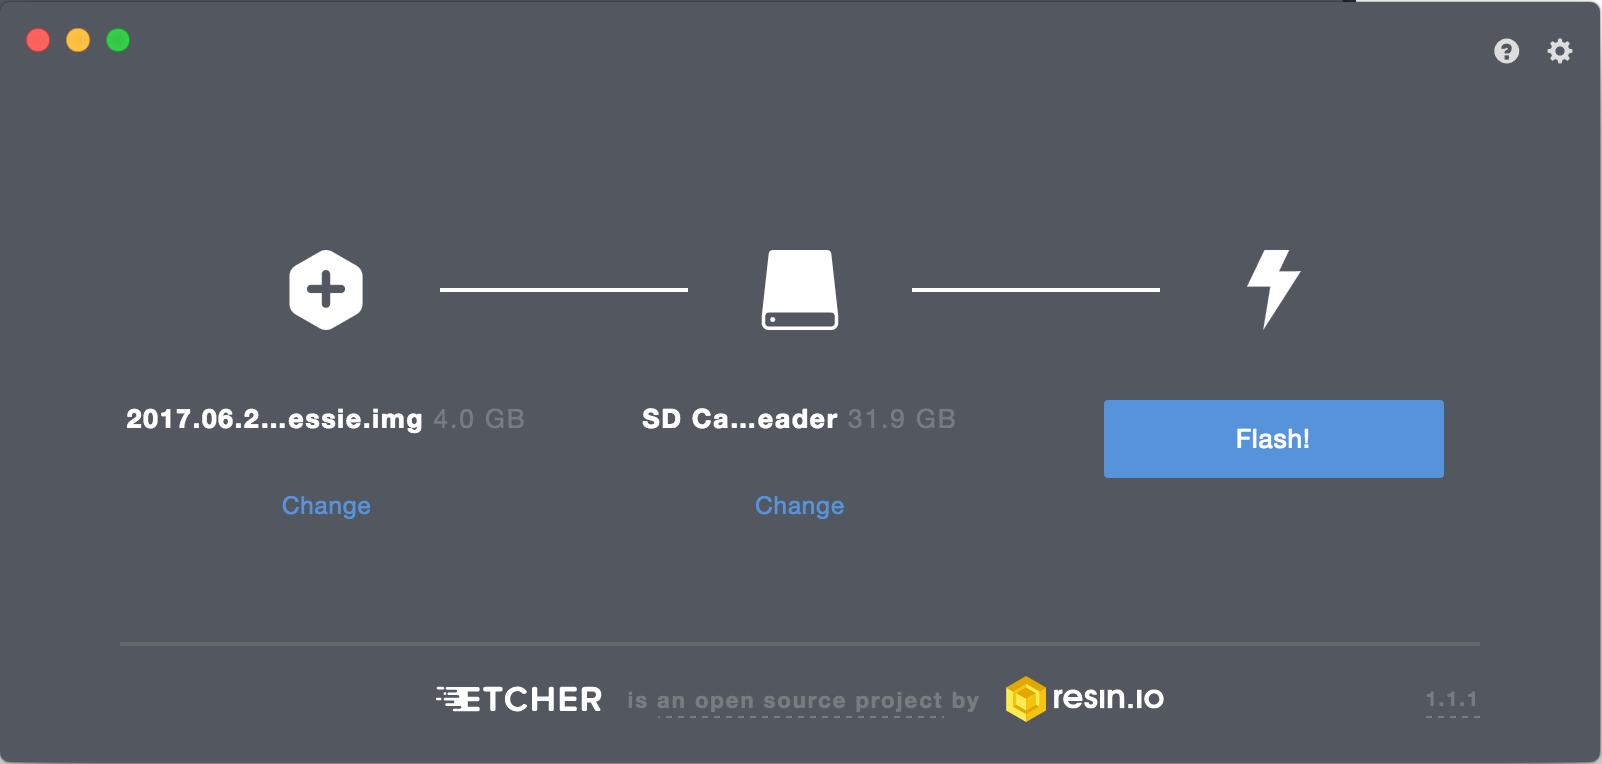
\includegraphics[width=0.5\textwidth]{images/etcher.png}
\caption{Etcher}
\end{figure}

\begin{enumerate}
\def\labelenumi{\arabic{enumi}.}
\setcounter{enumi}{3}

\item
  Eject your sd card and insert it into your raspberry pi.
\end{enumerate}

\section{Configure}\label{configure}

\subsection{Prepare OS}\label{prepare-os}

\section{Update}\label{update}

The following are essential updates:

\begin{verbatim}
sudo apt-get update
sudo apt-get upgrade
sudo apt-get install emacs
dpkg -l > ~/Desktop/packages.list
pip freeze > ~/Desktop/pip-freeze-initial.list
\end{verbatim}

The following are necessary for the scientific libraries, but they
require lots of space. Our sd cards do not have enough space for them.

\begin{verbatim}
sudo apt-get install build-essential python-dev python-distlib python-setuptools python-pip python-wheel libzmq-dev libgdal-dev
sudo apt-get install xsel xclip libxml2-dev libxslt-dev python-lxml python-h5py python-numexpr python-dateutil python-six python-tz python-bs4 python-html5lib python-openpyxl python-tables python-xlrd python-xlwt cython python-sqlalchemy python-xlsxwriter python-jinja2 python-boto python-gflags python-googleapi python-httplib2 python-zmq libspatialindex-dev
sudo pip install bottleneck rtree
\end{verbatim}

add to .bashrc

\begin{verbatim}
cd
git clone git://github.com/yyuu/pyenv.git .pyenv
echo 'export PYENV_ROOT="$HOME/.pyenv"' >> ~/.bashrc
echo 'export PATH="$PYENV_ROOT/bin:$PATH"' >> ~/.bashrc
echo 'eval "$(pyenv init -)"' >> ~/.bashrc
source ~/.bashrc

export PATH="/home/pi/.pyenv/bin:$PATH"
eval "$(pyenv init -)"
eval "$(pyenv virtualenv-init -)"

curl -L https://raw.githubusercontent.com/pyenv/pyenv-installer/master/bin/pyenv-installer | bash
\end{verbatim}

source

\subsection{Update to Python 3.6.1}\label{update-to-python-3.6.1}

\section{change python version}\label{change-python-version}

\begin{itemize}

\item
  {[}https://linuxconfig.org/how-to-change-from-default-to-alternative-python-version-on-debian-linux{]}
  (https://linuxconfig.org/how-to-change-from-default-to-alternative-python-version-on-debian-linux)
\end{itemize}

Upgrade setuptools for pip install with

\begin{verbatim}
    $ pip3 install --upgrade setuptools
    
\end{verbatim}

Test your python version with

\begin{verbatim}
    $ python --version
    
\end{verbatim}

Check your python version alternatives

\begin{verbatim}
    $ update-alternatives --list python
    
\end{verbatim}

If python2.7 is not in your alternatives, add it with

\begin{verbatim}
    $ sudo update-alternatives --install /usr/bin/python python /usr/bin/python2.7 1
    
\end{verbatim}

If python3.4 is not in your alternatives, add it with

\begin{verbatim}
    $ sudo update-alternatives --install /usr/bin/python python /usr/bin/python3.4 2
    
\end{verbatim}

Now make python3.4 to your default with

\begin{verbatim}
    update-alternatives --config python
\end{verbatim}

Select python3.4

\section{install 3.6.1}\label{install-3.6.1}

To install python 3.6.1, follow steps 1 and 2. This is unnecessary for
our purposes.

\begin{itemize}

\item
  \href{https://gist.github.com/dschep/24aa61672a2092246eaca2824400d37f}{better
  get 3.6.1}
\end{itemize}

\section{install cloudmesh.pi}\label{install-cloudmesh.pi}

pip install cloudmesh.pi

pip install cloudmesh.pi with

\begin{verbatim}
    $ git clone https://github.com/cloudmesh/cloudmesh.pi.git
    $ cd cloudmesh.pi
    $ sudo pip3 install .
\end{verbatim}

see how we do this in osx/linux can this be done on raspbery? if not
document update from source with altinstall

\subsection{Install scientific
Libraries}\label{install-scientific-libraries}

check if they are already installed we don't have enough space to
install all of these.

\begin{verbatim}
sudo apt-get install python-numpy python-matplotlib python-scipy python-sklearn python-pandas
\end{verbatim}

numpy\\
matplotlib\\
scipy\\
scikitlearn

\subsection{cloudmesh.pi (Jon)}\label{cloudmesh.pi-jon}

cloudmesh.pi is a repository for our GrovePi module classes. These
classes require Dexter software, so you need to either have Raspian for
Robots or download the software separately.

If you have Raspian for Robots, run the following in your terminal:

\begin{verbatim}
cd
mkdir github
cd github
git clone https://github.com/cloudmesh/cloudmesh.pi.git
cd cloudmesh.pi
sudo pip install .
\end{verbatim}

\subsection{Install VNC}\label{install-vnc}

describe how to install and configure VNC

\section{Sensors (Jon)}\label{sensors-jon}

\subsection{Grove Sensors (Jon)}\label{grove-sensors-jon}

we already have draft

\subsection{Non Grove Sensors (Jon)}\label{non-grove-sensors-jon}

Elegoo as example

\section{Notes To integrates}\label{notes-to-integrates}

\subsection{Connecting}\label{connecting}

Hostnames:

\begin{itemize}

\item
  raspberrypi.local
\item
  raspberrypi.
\end{itemize}

change

recovery.cmdline

forgot what these were:

\begin{verbatim}
runinstaller quiet ramdisk_size=32768 root=/dev/ram0 init=/init vt.cur_default=1 elevator=deadline
silentinstall runinstaller quiet ramdisk_size=32768 root=/dev/ram0 init=/init vt.cur_default=1 elevator=deadline
\end{verbatim}

Connect the cable

You will see the activity LEDs flash while the OS installs. Depending on
your SD-Card this can take up to 40-60 minutes.

\section{VLC on OSX}\label{vlc-on-osx}

\begin{itemize}
\item
  \url{http://www.videolan.org/vlc/index.en_GB.html}
\item
  \url{http://get.videolan.org/vlc/2.2.6/macosx/vlc-2.2.6.dmg}
\item
  \url{http://www.mybigideas.co.uk/RPi/RPiCamera/}
\item ~
  \section{Camera on Pi}\label{camera-on-pi}

  sudo apt-get install vlc
\item
  \url{https://www.raspberrypi.org/learning/getting-started-with-picamera/worksheet/}
\item
  \url{https://www.hackster.io/bestd25/pi-car-016e66}
\end{itemize}

\section{Streaming video}\label{streaming-video}

\begin{itemize}

\item
  \url{https://blog.miguelgrinberg.com/post/stream-video-from-the-raspberry-pi-camera-to-web-browsers-even-on-ios-and-android}
\end{itemize}

\section{Linux Commandline}\label{linux-commandline}

\begin{itemize}

\item
  \url{http://www.computerworld.com/article/2598082/linux/linux-linux-command-line-cheat-sheet.html}
\end{itemize}

\section{Enable SPI}\label{enable-spi}

go to the configuration interfaces and enable

\section{RTIMUlib2}\label{rtimulib2}

git clone https://github.com/RTIMULib/RTIMULib2.git cd RTIMULib

Add the following two lines to /etc/modules

\begin{verbatim}
i2c-bcm2708
i2c-dev
\end{verbatim}

reboot

\begin{verbatim}
ls /dev/i2c-*
sudo apt-get install i2c-tools

sudo i2cdetect -y 1
         0  1  2  3  4  5  6  7  8  9  a  b  c  d  e  f
00:          -- -- -- -- -- -- -- -- -- -- -- -- -- 
10: -- -- -- -- -- -- -- -- -- -- -- -- -- -- -- -- 
20: -- -- -- -- -- -- -- -- -- -- -- -- -- -- -- -- 
30: -- -- -- -- -- -- -- -- -- -- -- -- -- -- -- -- 
40: -- -- -- -- -- -- -- -- -- -- -- -- -- -- -- -- 
50: -- -- -- -- -- -- -- -- -- -- -- -- -- -- -- -- 
60: -- -- -- -- -- -- -- -- 68 -- -- -- -- -- -- -- 
70: -- -- -- -- -- -- -- --
\end{verbatim}

\begin{figure}[htb]
\centering
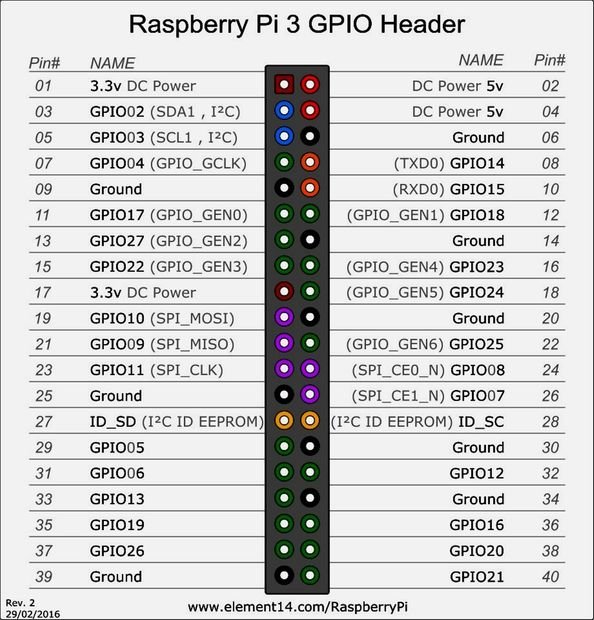
\includegraphics[width=0.5\textwidth]{images/rasp3.jpg}
\caption{Pinout}
\end{figure}

create a file /etc/udev/rules.d/90-i2c.rules and add the line:

\begin{verbatim}
KERNEL=="i2c-[0-7]",MODE="0666"
\end{verbatim}

note: does not work

instead we do

\begin{verbatim}
sudo chmod 666 /dev/i2c-1 
\end{verbatim}

Set the I2C bus speed to 400KHz by adding to /boot/config.txt:

\begin{verbatim}
dtparam=i2c1_baudrate=400000
\end{verbatim}

reboot. In terminal change directories to

\begin{verbatim}
cd /home/pi/github/RTIMULib2/RTIMULib/IMUDrivers
\end{verbatim}

and open

\begin{verbatim}
emacs RTIMUDefs.h
\end{verbatim}

In RTIMUDefs.h change

\begin{verbatim}
#define MPU9250_ID 0x71
\end{verbatim}

To

\begin{verbatim}
#define MPU9250_ID 0x73



cd /home/pi/github/RTIMULib2/RTIMULib
\end{verbatim}

In terminal

\begin{verbatim}
mkdir build
cd build
cmake ..
make -j4
sudo make install
sudo ldconfig
\end{verbatim}

\section{Compile RTIMULib Apps}\label{compile-rtimulib-apps}

\begin{verbatim}
cd /home/pi/github/RTIMULib2/Linux/RTIMULibCal
make clean; make -j4
sudo make install
cd /home/pi/github/RTIMULib2/Linux/RTIMULibDrive
make clean; make -j4
sudo make install
cd /home/pi/github/RTIMULib2/Linux/RTIMULibDrive10
make clean; make -j4
sudo make install
cd /home/pi/github/RTIMULib2/Linux/RTIMULibDrive11
make clean; make -j4
sudo make install


cd /home/pi/github/RTIMULib2/Linux/RTIMULibDemo    
qmake clean
make clean
qmake
make -j4
sudo make install
cd /home/pi/github/RTIMULib2/Linux/RTIMULibDemoGL
qmake clean
make clean
qmake
make -j4
sudo make install
\end{verbatim}

\section{Camera}\label{camera}

\begin{itemize}

\item
  \href{https://www.raspberrypi.org/learning/getting-started-with-picamera/worksheet/}{Camera
  Tutorial}
\end{itemize}

.

\begin{verbatim}
sudo apt-get install libjpeg-dev libtiff5-dev libjasper-dev libpng12-dev
sudo apt-get install libavcodec-dev libavformat-dev libswscale-dev libv4l-dev

sudo apt-get install libxvidcore-dev libx264-dev

sudo pip install virtualenv virtualenvwrapper
sudo rm -rf ~/.cache/pip
\end{verbatim}

copy into \textasciitilde{}/.profile:

\begin{verbatim}
 echo -e "\n# virtualenv and virtualenvwrapper" >> ~/.profile
 echo "export WORKON_HOME=$HOME/.virtualenvs" >> ~/.profile
 echo "source /usr/local/bin/virtualenvwrapper.sh" >> ~/.profile
\end{verbatim}
%$

source \textasciitilde{}/.profile

\begin{verbatim}
mkvirtualenv cv -p python3
\end{verbatim}

workon cv

comandline has (cv) in front

\begin{verbatim}
pip install numpy

wget -O opencv.zip https://github.com/Itseez/opencv/archive/3.1.0.zip
wget -O opencv_contrib.zip https://github.com/Itseez/opencv_contrib/archive/3.1.0.zip
unzip opencv.zip
unzip opencv_contrib.zip
\end{verbatim}

\section{Lessons and Projects}\label{lessons-and-projects}

\begin{itemize}

\item
  \href{https://www.raspberrypi.org/learning/getting-started-with-guis/worksheet/}{Gui}\\
\item
  \href{https://www.raspberrypi.org/learning/getting-started-with-guis/}{Solder}\\
\item
  \href{https://www.raspberrypi.org/blog/an-image-processing-robot-for-robocup-junior/}{PI
  Camera Line Follower}\\
\item
  \href{https://circuitdigest.com/microcontroller-projects/web-controlled-raspberry-pi-surveillance-robot}{Pi
  car flask}
\end{itemize}

\section{OTHER TO BE INTEGRATED}\label{other-to-be-integrated}

\subsection{PI emulator on Windows}\label{pi-emulator-on-windows}

We have not yet tried it, but we like to hear back from you on
experiences with

\begin{itemize}

\item
  https://sourceforge.net/projects/rpiqemuwindows/
\end{itemize}

\subsection{Scratch}\label{scratch}

\begin{itemize}

\item
  \href{https://github.com/DexterInd/GrovePi/tree/master/Software/Scratch}{scratch}
\end{itemize}

\section{Web Server}\label{web-server}

\begin{itemize}

\item
  \href{https://www.raspberrypi.org/learning/python-web-server-with-flask/worksheet/}{Web
  Server Flask}
\end{itemize}
